\documentclass[12pt,a4paper, titlepage]{article}
\usepackage{tikz}
\usetikzlibrary{arrows}
\usetikzlibrary{bayesnet}
\usepackage{amsmath}
\usepackage{bm}
\usepackage{xcolor}
\usepackage[left=2.00cm, right=2.00cm, top=2.00cm, bottom=2.00cm]{geometry}
\author{}
\title{}

\newcommand{\age}{\mbox{age}}
\newcommand{\male}{\mbox{male}}
\newcommand{\creat}{\mbox{creat}}
\newcommand{\wt}{\mbox{wt}}
\newcommand{\harpoon}{\overset{\rightharpoonup}}
\begin{document}



\begin{figure}[t!]
	
\centering
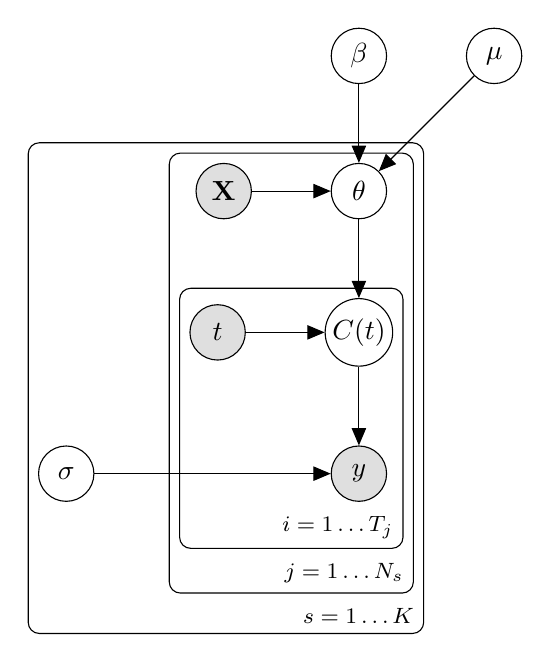
\begin{tikzpicture}
	
\node[latent](b){$\beta$};
\node[latent, right=of b](mu){$\mu$};

\node[latent, below = of b](theta){$\theta$};
\node[obs, left = of theta](x){$\mathbf{X}$};


\node[latent, below = of theta](C){$C(t)$};
\node[obs, left = of C](t){$t$};
\node[obs, below = of C](y){$y$};
\node[latent, left = of y, xshift=-2cm](s){$\sigma$};

\edge{b}{theta};
\edge{mu}{theta};
\edge{x}{theta};
\edge{theta}{C};
\edge{t}{C};
\edge{C}{y};
\edge{s}{y};

\plate[]{t_y_pairs}{(t)(y)(C)}{$i=1 \dots T_j$};
\plate[]{subjects}{(t_y_pairs)(x)(theta)}{$j=1 \dots N_s$};
\plate[]{study}{(subjects)(s)}{$s=1 \dots K$};
\end{tikzpicture}
\end{figure}

\end{document}

%
%\begin{figure}[t!]
%	
%	\centering
%	\begin{tikzpicture}
%	\node[latent](b){$\boldsymbol{\beta}$};
%	\node[latent, below= of b, yshift=-2cm](mu){$\boldsymbol{\mu}$};
%	
%	\node[latent, left= of b, yshift=1cm](r_Cl){$Cl$};
%	\node[latent, left= of b, yshift=-1cm](r_t){$t_{\max}$};
%	\node[latent, left= of mu, yshift=1cm](r_a){$\alpha$};
%	\node[latent, left=of mu, yshift=-1cm](r_F){$F$};
%	
%	\edge{b}{r_Cl};
%	\edge{b}{r_t};
%	\edge{b}{r_a};
%	\edge{mu}{r_Cl};
%	\edge{mu}{r_t};
%	\edge{mu}{r_a};
%	\edge{mu}{r_F};
%
%   	\node[latent, left= of r_t](r_C){$C(t)$};
%   	
%   	\edge{r_Cl}{r_C};
%   	\edge{r_t}{r_C};
%   	\edge{r_a}{r_C};
%     \edge{r_F}{r_C};
%   	
%   	
%   	\node[obs, left= of r_C](r_y){$y$};
%   	\node[obs, below= of r_C](r_time){$t$};
%   	\node[latent, above=of r_C](delay){$ \delta $};
%   	
%   	\edge{r_time}{r_C};
%   	 \edge{delay}{r_C};
%   	\edge{r_C}{r_y};
%   	
%   	\node[latent, left= of r_y, xshift=-1cm](r_sigma){$\sigma_1$};
%   	
%   	\edge{r_sigma}{r_y};
%   	
%	\plate[]{t_y_pairs}{(r_time)(r_y)(r_C)}{$i=1\dots8$};
%	\plate{rommel_model}{(t_y_pairs)(r_C)(r_Cl)(r_t)(r_a)(r_F)}{$j = 1\dots 36$};
%
%	
%	\node[latent, right= of b, yshift=1cm](u_Cl){$Cl$};
%	\node[latent, right= of b, yshift=-1cm](u_t){$t_{\max}$};
%	\node[latent, right= of mu, yshift=1cm](u_a){$\alpha$};
%	\node[latent, right= of mu, yshift=-1cm](u_F){$F$};
%		
%	\edge{b}{u_Cl};
%	\edge{b}{u_t};
%	\edge{b}{u_a};
%	\edge{b}{u_F};
%	\edge{mu}{u_Cl};
%	\edge{mu}{u_t};
%	\edge{mu}{u_a};
%   \edge{mu}{u_F};
%	
%
%	\node[latent, right= of u_t](u_C){$C(t)$};
%	
%	  \edge{u_Cl}{u_C};
%	\edge{u_t}{u_C};
%	\edge{u_a}{u_C};
%	\edge{u_F}{u_C};
%	
%	\node[obs, right= of u_C](u_y){$y$};
%		
%	\node[obs, below= of u_C](u_time){$t$};
%	\node[latent, right= of u_y, xshift=1cm](u_sigma){$\sigma_2$};
%	
%	\edge{u_time}{u_C};
%	\edge{u_C}{u_y};
%	\edge{u_sigma}{u_y};
%	
%	\plate[color=blue]{experimental}{(b)(mu)(rommel_model)(r_sigma)}{\color{blue}{Experimental Model}};
%	\plate[color=red]{observational}{(b)(mu)(u_Cl)(u_t)(u_a)(u_F)(u_C)(u_time)(u_y)(u_sigma)}{\color{red}{Observational Model}};
%	\end{tikzpicture}
%
%\end{figure}
%
%
%\end{document}